\section{Compiler Design}
\labsec{ch05-compiler-design}
There were several elements that conditioned the architecture of this system. First of all,
there is no database or data access layer that needs to be taken into account. There isn’t
also any presentation or visual interface of data other from the CLI. The system consists
mainly of functionality that is offered to other users to use from the CLI or create their own
systems. 

All of these elements simplified noticeably the architecture of the system. \reffig{shex-lite-high-level-arch} sumarizes the high level architecture of the ShEx-Lite compiler. Notice that the elements that appear here are the same that where identified in \refch{compiler-analysis}.

\begin{figure}[hb]
    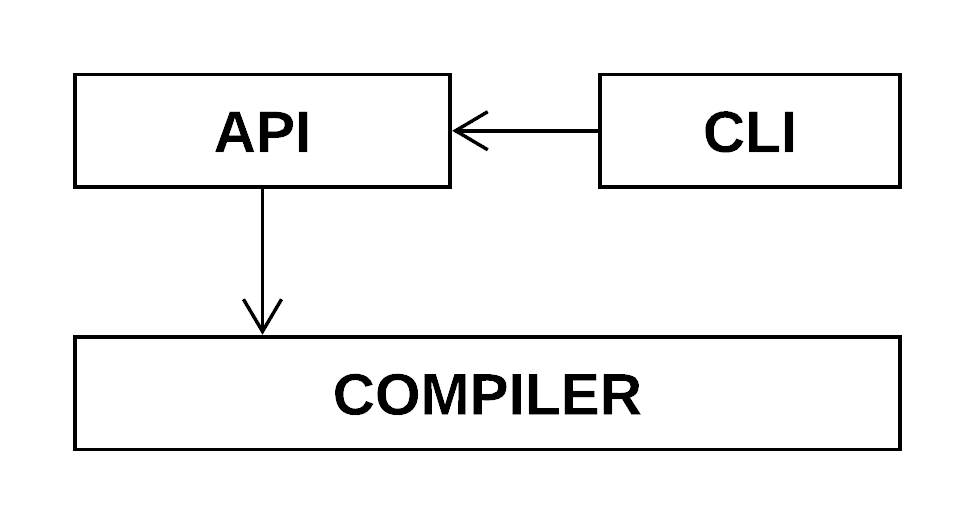
\includegraphics{shex-lite-high-level-arch.png}
    \caption[High level view of the ShEx-Lite system]{High level view of the ShEx-Lite system. This figure shows how the CLI is build on top of the API which depends on the compiler implementation.}
    \labfig{shex-lite-high-level-arch}
\end{figure}

\begin{figure}[hb]
    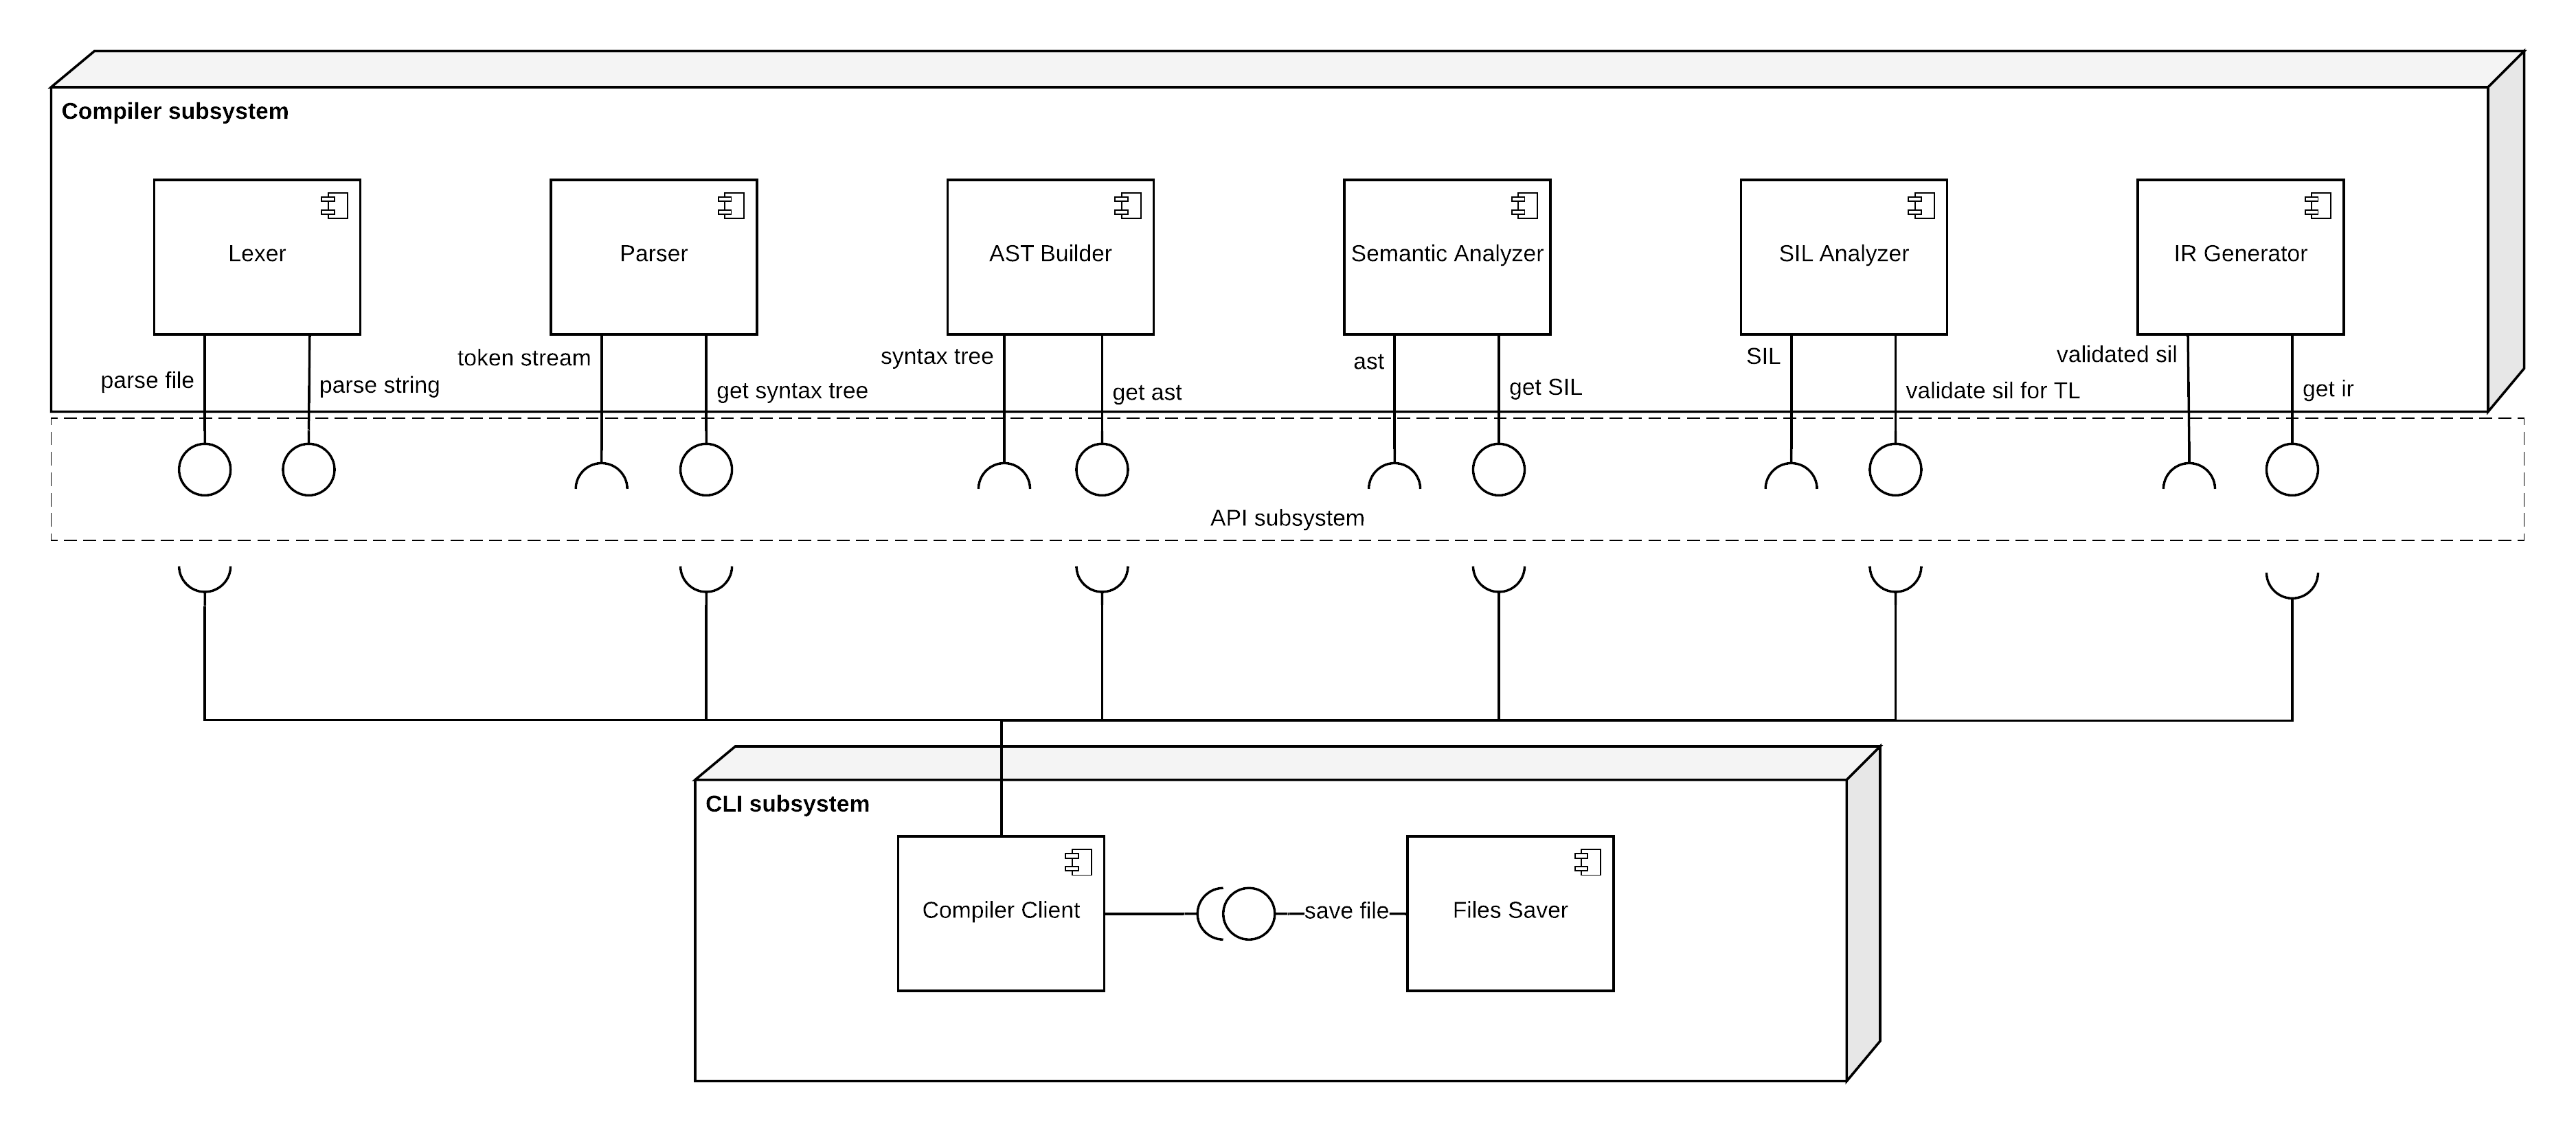
\includegraphics{shex-lite-components.png}
    \caption[Components diagram for ShEx-Lite Compiler]{Components diagram for ShEx-Lite Compiler.}
    \labfig{shex-lite-components}
\end{figure}

\reffig{shex-lite-components} shows the three main subsystems that the ShEx-Lite compiler contains, the
compiler itself, the API composed by the interfaces that the compiler exposes and the CLI
subsystem that acts as a client implementation of the API subsystem.
At this point it is important to take a moment to explain the architectural pattern that ShExLite employs. From the beginning we introduce the pattern “compiler as an API”, this
pattern is perfectly explained in the Theoretical Background and it affects the design of the
system in the following way.
Each component of the compiler subsystem can be executed independently of the others,
exposing an interface and producing and output. This produces a subsystem that does not
contain any implementation but requires the highest effort for a good design, the API
subsystem.
Now we will explore the architecture of the three subsystems independently.

\subsection{Compiler}
The compiler contains the implementation for the API interfaces. Its task is to give the
functionality to the designed interfaces, to do so it implements different programming
patterns.

\begin{figure}[hb]
    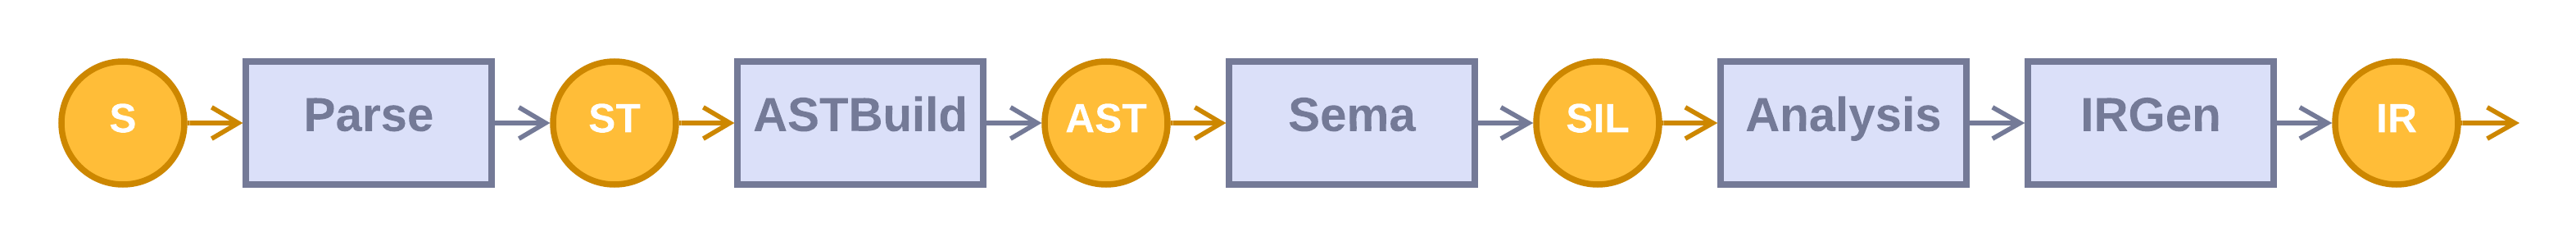
\includegraphics{shex-lite-process-01.png}
    \caption[High level view of the compiler flow]{High level view of the compiler flow.}
    \labfig{shex-lite-process-01}
\end{figure}

The \reffig{shex-lite-process-01} shows from a very high point of view a complete sequence of compilation
for the ShEx-Lite compiler. From there we can already capture that the compiler will be
composed of the following elements: 

\begin{itemize}
    \item \textbf{Parse:} Takes as input the source files and produces the Syntax Tree. 
    \item \textbf{ASTBuild:} Takes as an input the Syntax Tree and generates an Abstract Syntax Tree.
    \item \textbf{Sema:} From the Abstract Syntax Tree generated in the previous step it produces the ShEx-Lite Intermediate Language.
    \item \textbf{SIL Analysis:} Analyses the ShEx-Lite intermediate code and decides whether the corresponding Intermediate Representation can be dispatched or not.
    \item \textbf{IRGen:} Generates the corresponding Intermediate Representation.
\end{itemize}

Notice that those elements are independent one from another. Also from the \reffig{shex-lite-process-01}
we can already extract that the compiler will have at least the following structures:

\begin{itemize}
    \item \textbf{S:} Holds the Sources that the compiler will process. Those sources are \texttt{.shexl} files that contain the schemas that the user wants to compile.
    \item \textbf{ST:} Holds the output of the parse process. The parse process produces the Syntax Tree but also might generate warnings and errors. 
    \item \textbf{AST:} Contains the output of building the AST. This AST has not been type-checked nor annotated. 
    \item \textbf{SIL:} Contains the ShEx-Lite Intermediate Language. The SIL is the name for the typechecked annotated AST that has been transformed in to a graph structure. But it might also contains semantic error / warnings. 
    \item \textbf{IR:} Contains the generated Intermediate Representation. The IR is the sources that represent the generated domain object model, it contains those sources and all the compilation information. 
\end{itemize}

\begin{figure*}[hb]
    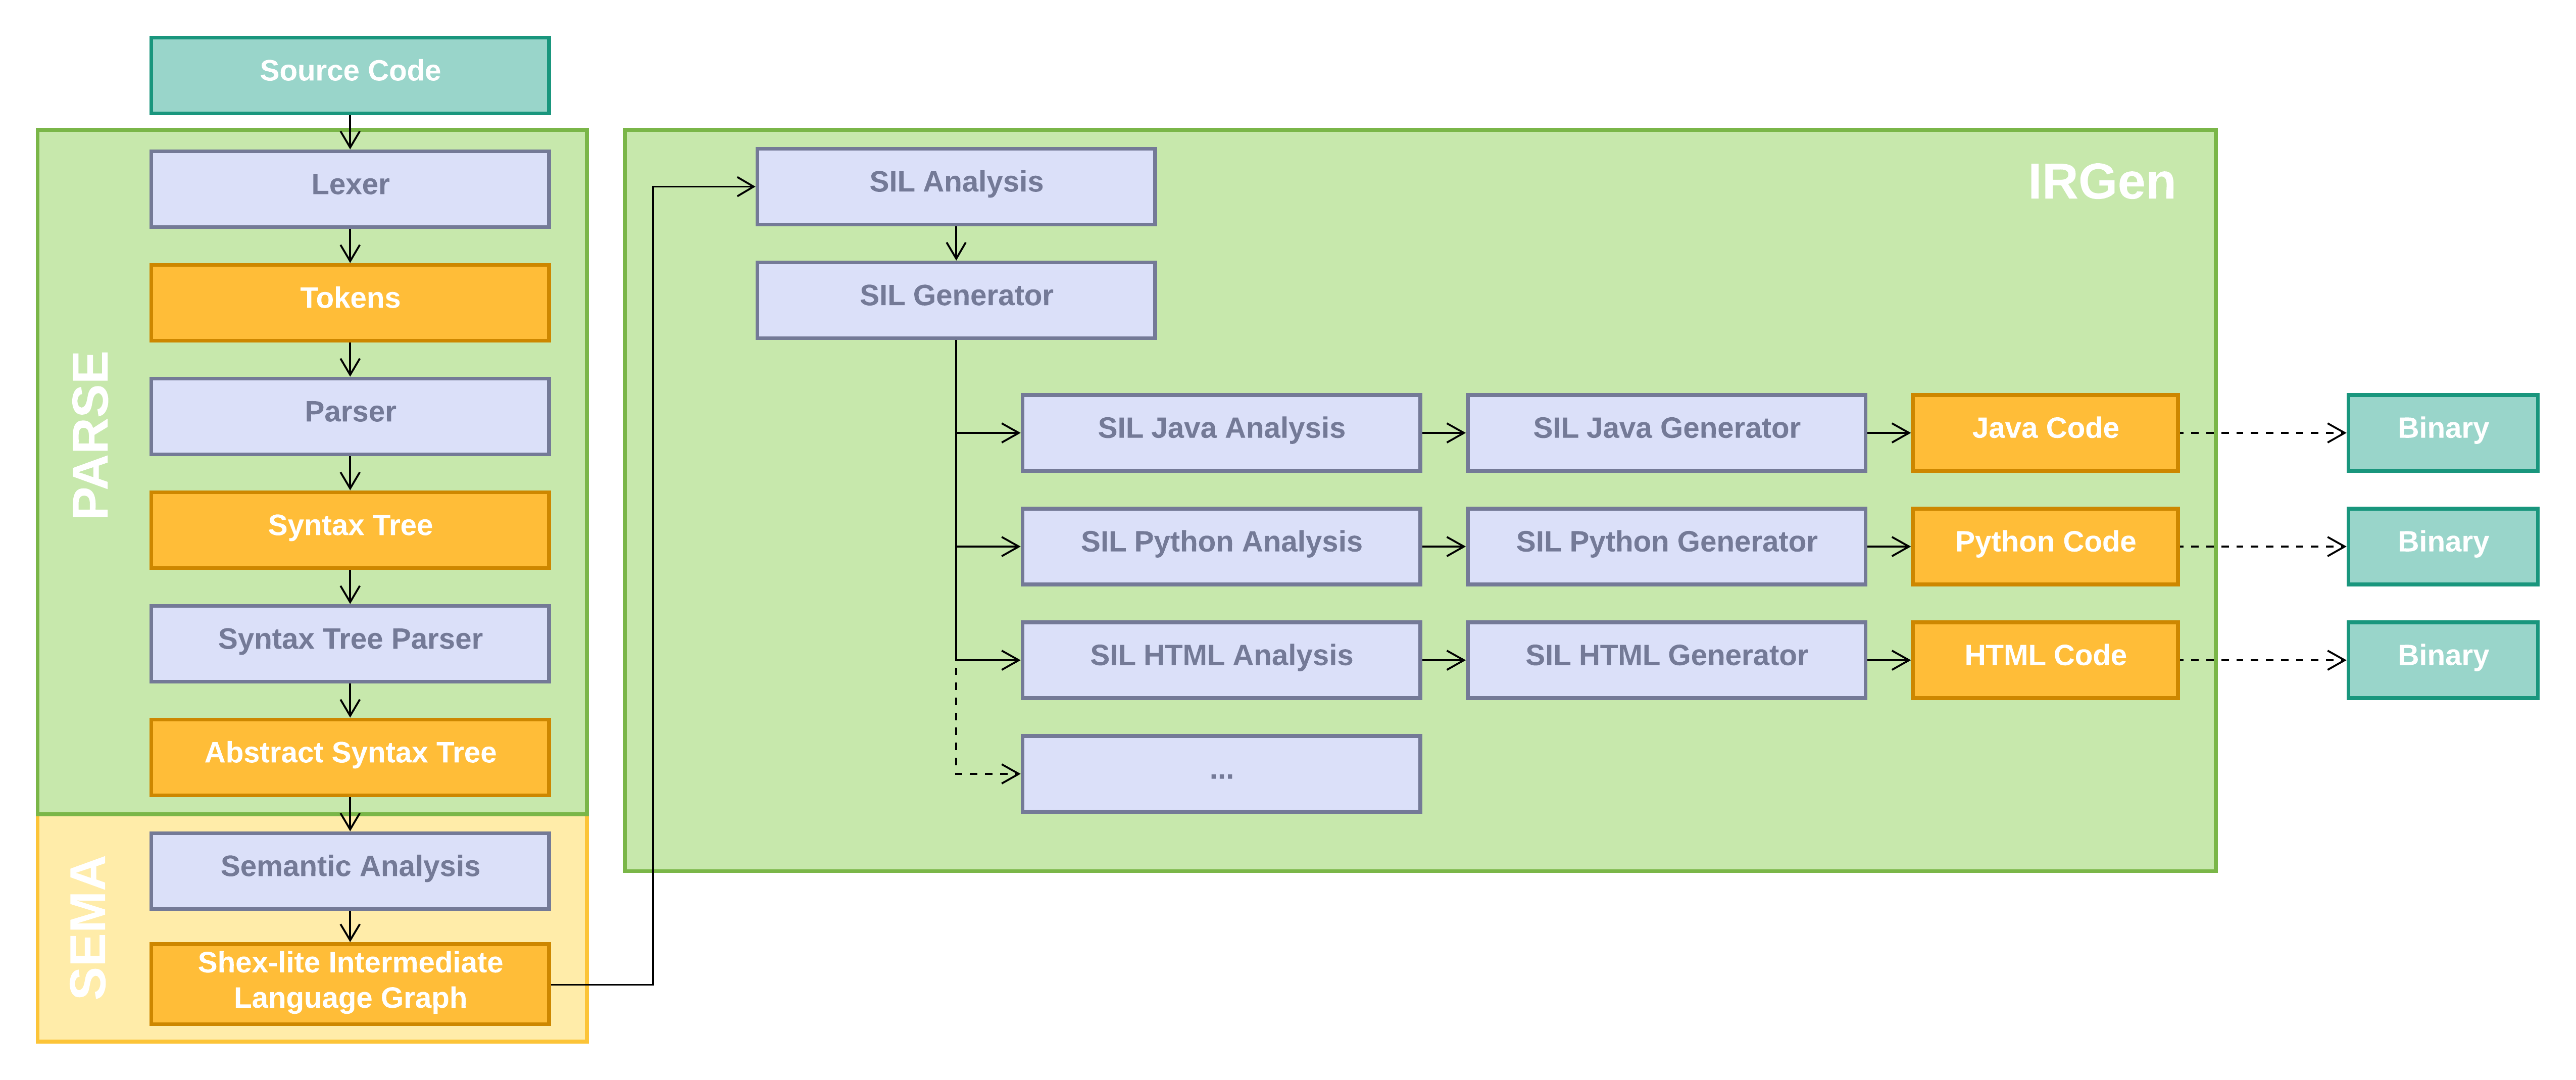
\includegraphics{shex-lite-process-02.png}
    \caption[Low level view of the compiler flow, grouped by compiler-action]{Low level view of the compiler flow, grouped by compiler-action.}
    \labfig{shex-lite-process-02}
\end{figure*}

From the \reffig{shex-lite-process-02} we can see that in the compiler each process (Parse, sema, …)
contains multiple components. For example the parse stage from \reffig{shex-lite-process-01} is composed
by a lexer and a parser, that will correspond with the first two components of the compiler
subsystem from \reffig{shex-lite-components}. This components will be deeply explored at the class diagram
section. 